\documentclass[12pt,preprint]{aastex}

\usepackage{amsmath}
\def\half{{\textstyle\frac12}}

\begin{document}

\title{Lens Modeling in Spacewarps}

\author{First Author,\altaffilmark{1}
Second Author,\altaffilmark{2} and
Third Author\altaffilmark{3}}
\altaffiltext{1}{First place}
\altaffiltext{2}{Second place}
\altaffiltext{3}{Third place}

\begin{abstract}
In Spacewarps, volunteers are invited to search sky surveys for lens
candidates.  Here we report on a system that allows experienced
volunteers to model lens candidates.  A sample of 29 simulated lenses
were modelled, each multiple times.  The quality of the models was
then examined in two ways.  First, the image parities and time
orderings: these were identified correctly in most cases, but not
always.  Second, the mean convergence (equivalent to the enclosed
mass): this was constrained consistently well in the image region.
The performance of professionals and experienced volunteers was
comparable.
\end{abstract}

\keywords{}

\section{Introduction}

Spacewarps is the future.

Moreover, that lens modelling is an essential accompaniment to lens
searches has been clear since the early days \citep{1981ApJ...244..723Y}.

Why Fermat's principle?  Details in \ref{sec:Fermat} and
\ref{sec:more-theory}.

SpaghettiLens details in \ref{sec:SpaghettiLens}.

Sims in \ref{sec:sims}.

Results in \ref{sec:results}.

Things to do in \ref{sec:todo}.

\section{Fermat's Principle} \label{sec:Fermat}

Explain Fermat's principle
\begin{equation}
\hbox{arrival time} = A_{\rm geom} - A_{\rm grav}
\end{equation}
By convention, $A_{\rm grav}$ is defined in such a way that it is
negative, hence the minus sign.

Although $A_{\rm geom}$ and $A_{\rm grav}$ are times, we are going to
write them as if they are areas.  In other words, we will suppress a
constant factor in the $A$.  That factor is basically the lens
distance times the speed of light, but the precise expression is given
in the Appendix.

Introduce the Laplacian $\nabla^2 f(x,y)$ is
\begin{equation}
 \frac{ f(x+\Delta x, y) + f(x-\Delta x, y) +
        f(x, y+\Delta y) + f(x, y-\Delta y) - 4 f(x,y) }
      {\Delta x \; \Delta y}
\end{equation}
in the limit of $\Delta x,\Delta y$ small.

Let $x,y$ be coordinates on the lens, transverse to the line of sight.
Let there be a point source behind $x=0,y=0$.  Then
\begin{equation}
A_{\rm geom}(x,y) = \half(x^2 + y^2)
\end{equation}
\begin{equation}
\nabla^2 A_{\rm grav}(x,y) = 2\kappa(x,y)
\end{equation}
Here $\kappa$ is a dimensionless quantity with two distinct physical
interpretations.  On the one hand, it is the sky projected density ---
in special units, to make it dimensionless.  On the other hand,
$\kappa$ is the {\em convergence\/} of a bundle of rays.

\section{SpaghettiLens} \label{sec:SpaghettiLens}

Give a guess for the maximum, minimum and saddle points.  Program
tries find $\kappa(x,y)$ that reproduces these properties exactly, and
looks reasonably like a galaxy.  Solution not unique, an ensemble
generated.

\section{The simulated lenses} \label{sec:sims}

Three kinds of sims.

\begin{itemize}
\item {\em Quasar:\/} A singular elliptical isothermal plus constant
  external shear, with a circular Gaussian source.
\item {\em Galaxy:\/} Lens as with quasar, but elliptical de
  Vaucouleurs source.
\item {\em Galaxy:\/} Lens is circular NFW plus one dominant
  elliptical SIE and perturbating elliptical SIEs, source as with
  galaxy.
\end{itemize}
Lenses follow \cite{2001astro.ph..2341K,2001astro.ph..2340K}.
Parameters in online supplement.

\section{Results} \label{sec:results}

Example Figure \ref{fig:ASW0000ar2}.

\section{Extensions needed} \label{sec:todo}

\appendix

\section{More on Lensing Theory} \label{sec:more-theory}

First we define comoving distances, as follows.
\begin{equation}
\int \frac{dz}{\sqrt{\Omega_m(1+z)^3 + \Omega_\Lambda}}
\end{equation}
\begin{equation}
\begin{aligned}
&D_S    &                                &\int_0^{a_S} \\
\noalign{\medskip}
&D_{LS} & = \frac c{H_0} \ \times \quad  &\int_{z_L}^{z_S} \\
\noalign{\medskip}
&D_L    &                                &\int_0^{z_L}
\end{aligned}
\end{equation}

\begin{equation}
\begin{aligned}
A           &= cD_L \frac{D_{LS}}{D_S} \times t \\
\kappa(x,y) &= \frac{4\pi G}{c^2} \frac{D_L}{1+z} \frac{D_{LS}}{D_S}
               \times \Sigma(x,y)
\end{aligned}
\end{equation}

Let $x,y$ be physical distances on the lens plane and $D_L$ be
comoving distances.  Then
\begin{equation}
t_{\rm geom} = \frac{(1+z_L)^2}{2cD_L} \frac{D_S}{D_{LS}}
\left( (x-s_x)^2 + (y-s_y)^2 \right)
\end{equation}
\begin{equation}
\nabla^2 t_{\rm grav} = (1+z_L)\frac{8\pi G}{c^3} \, \Sigma(x,y)
\end{equation}

Can replace comoving distances $D$ with angular-diameter distances
$d$,
\begin{equation}
(x,y) = d_L (\theta_x,\theta_y)
\end{equation}
and so on.
\begin{equation}
\begin{aligned}
D_S &= (1+z_S) \, d_S \\
D_{LS} &= \frac{1+z_S}{1+z_L} \, d_{LS} \\
D_L &= (1+z_L) \, d_L
\end{aligned}
\end{equation}
Angular-diameter distances are always smaller than comoving distances.

Recover equations (2.1) to (2.6) from \cite{1986ApJ...310..568B}.

\newpage

\bibliographystyle{apj}
\bibliography{ms}

\newpage


\begin{figure}
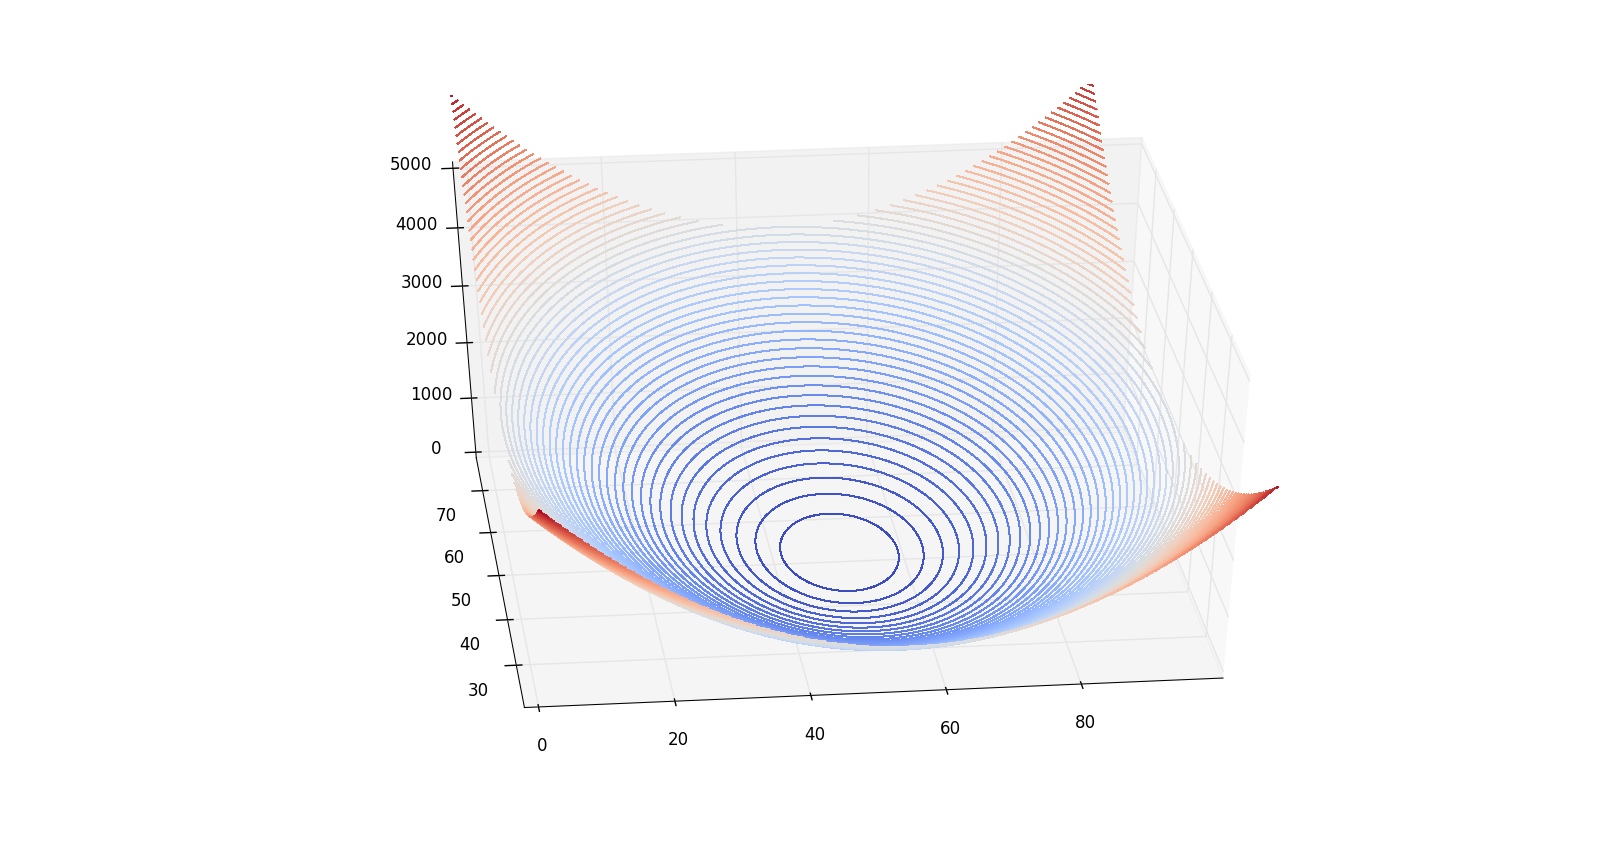
\includegraphics[height=.3\vsize]{arriv1.png}
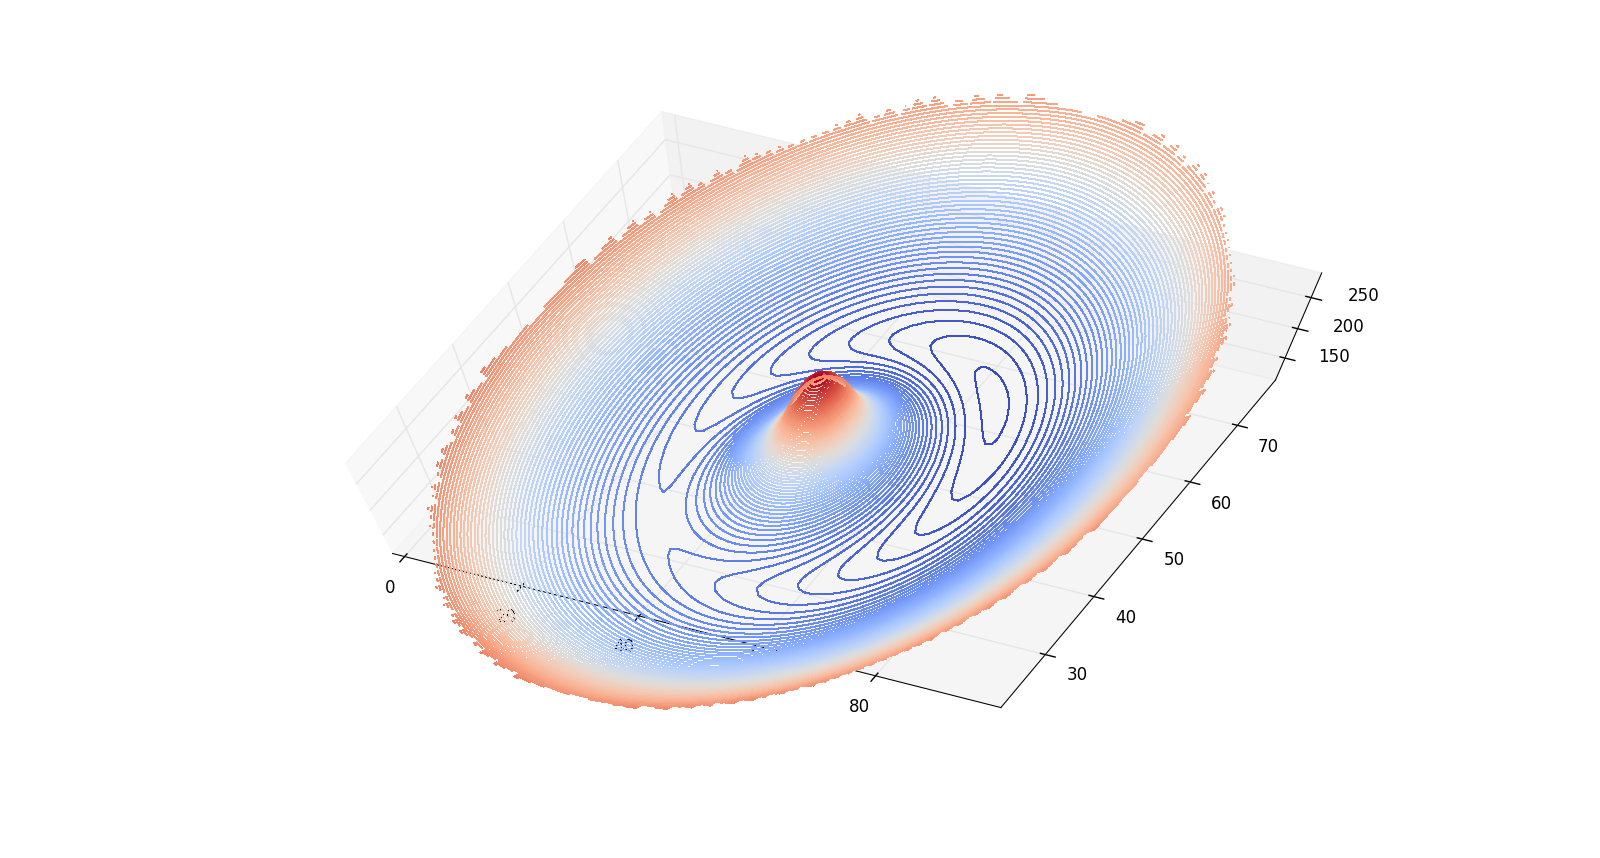
\includegraphics[height=.3\vsize]{arriv2.png}
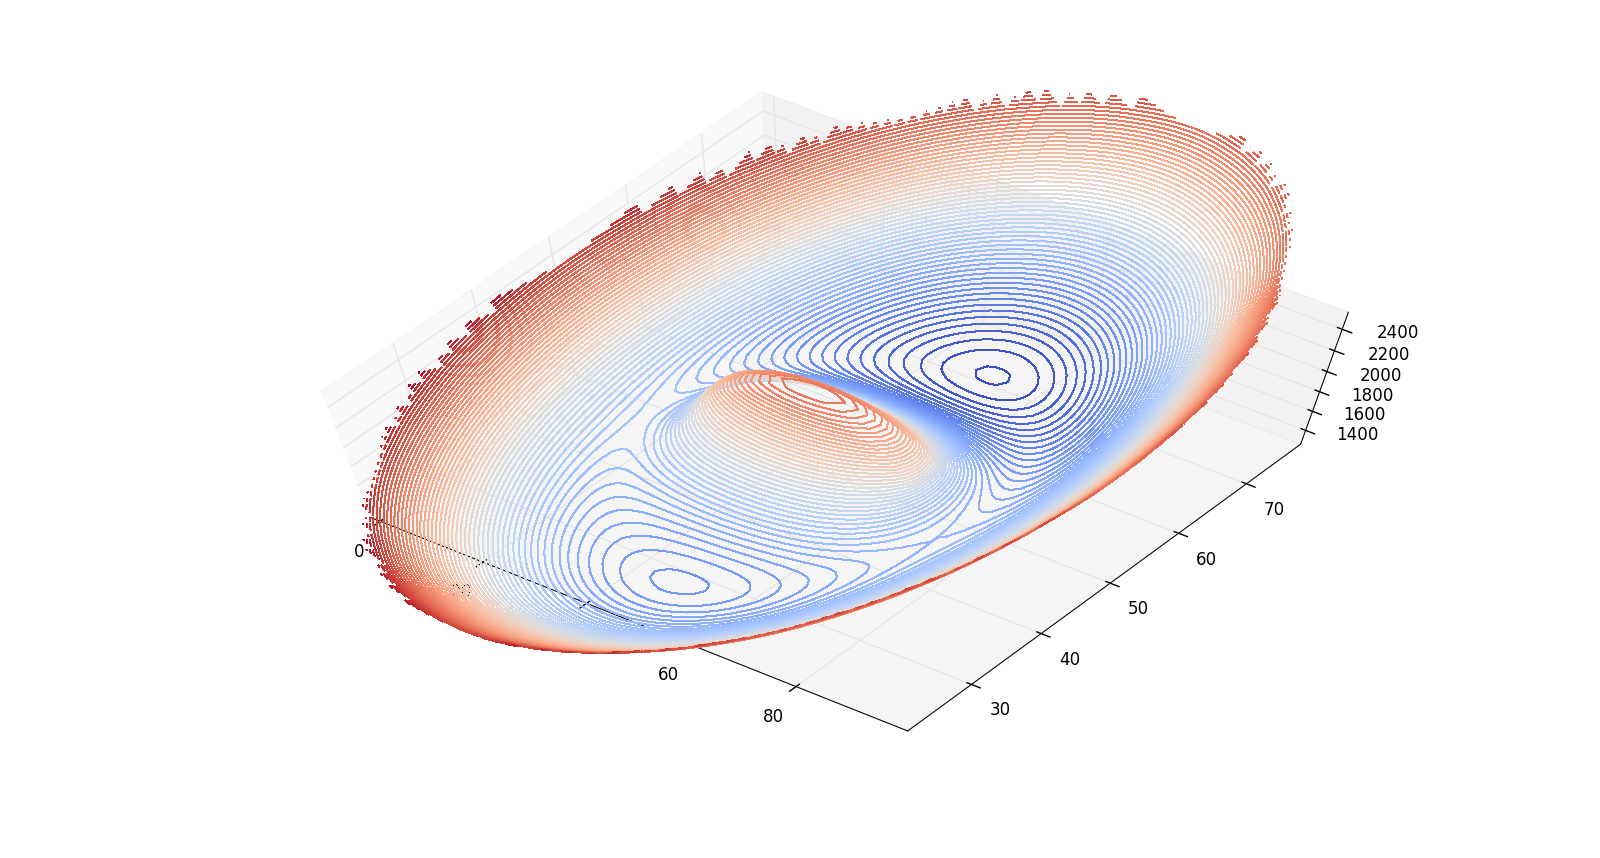
\includegraphics[height=.3\vsize]{arriv3.png}
\caption{Arrival-time surfaces\label{fig:arriv}}
\end{figure}

\begin{figure}
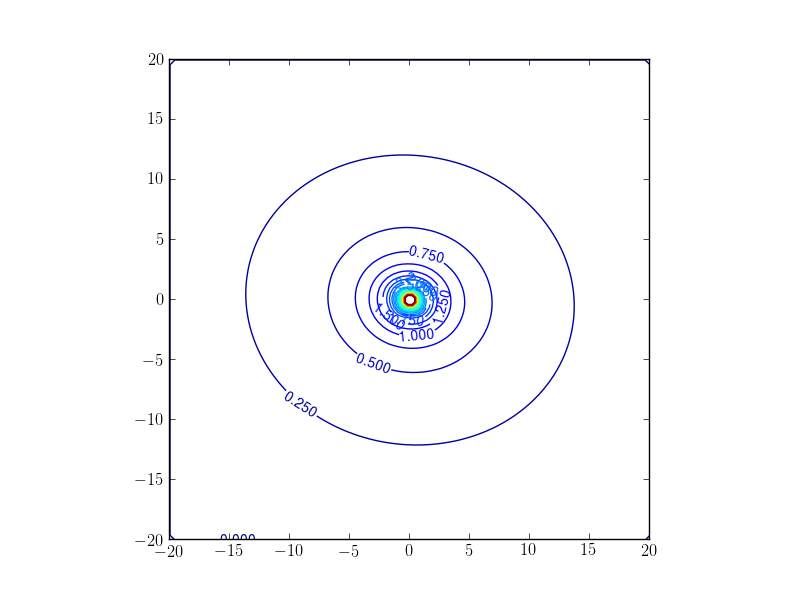
\includegraphics[width=.32\hsize]{ASW0000ar2Q_kappa.png}
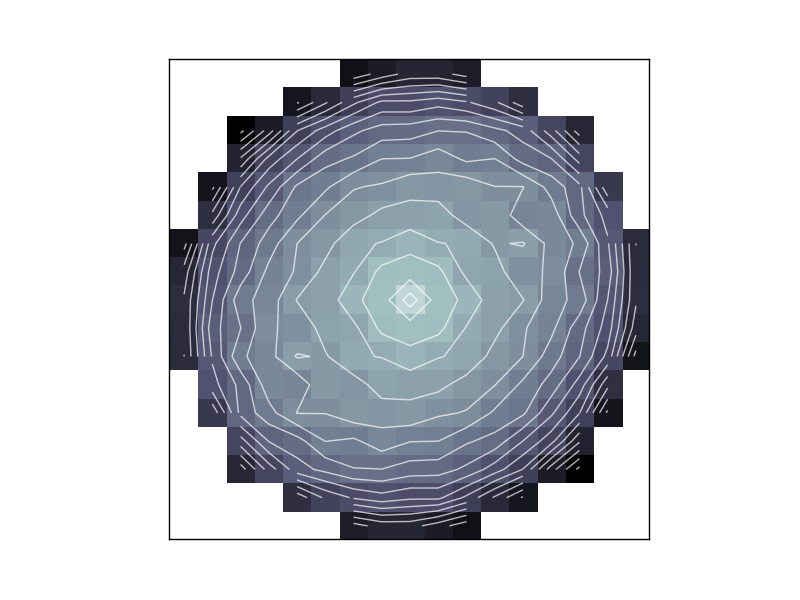
\includegraphics[width=.32\hsize]{ASW0000ar2_kappa.png}
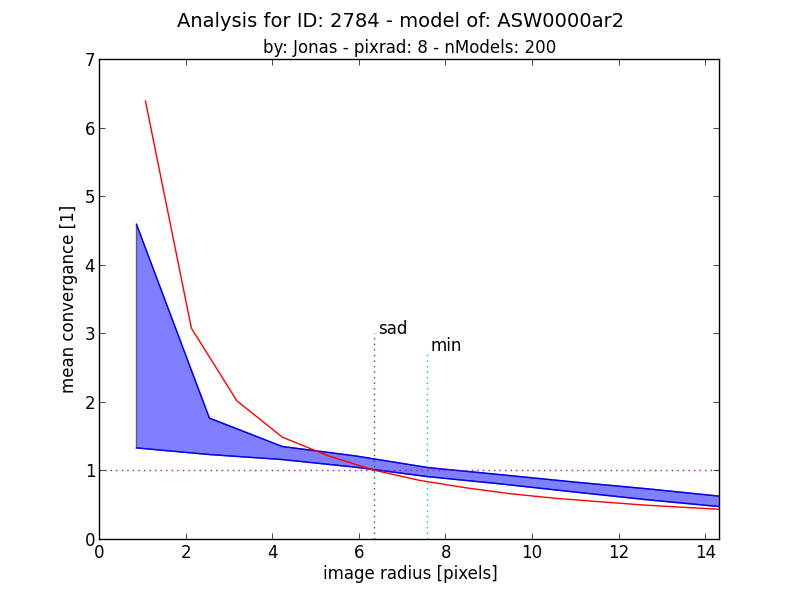
\includegraphics[width=.32\hsize]{ASW0000ar2_menc.png} \\
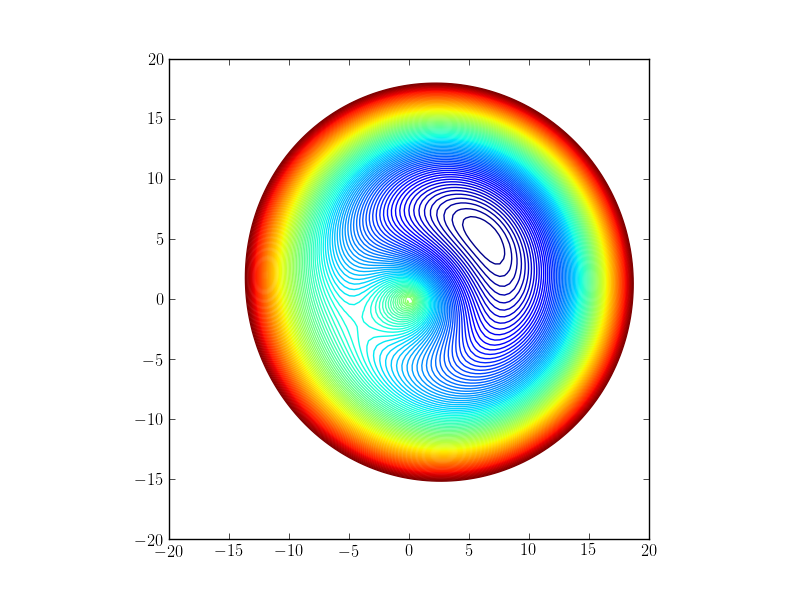
\includegraphics[width=.32\hsize]{ASW0000ar2Q_arriv.png}
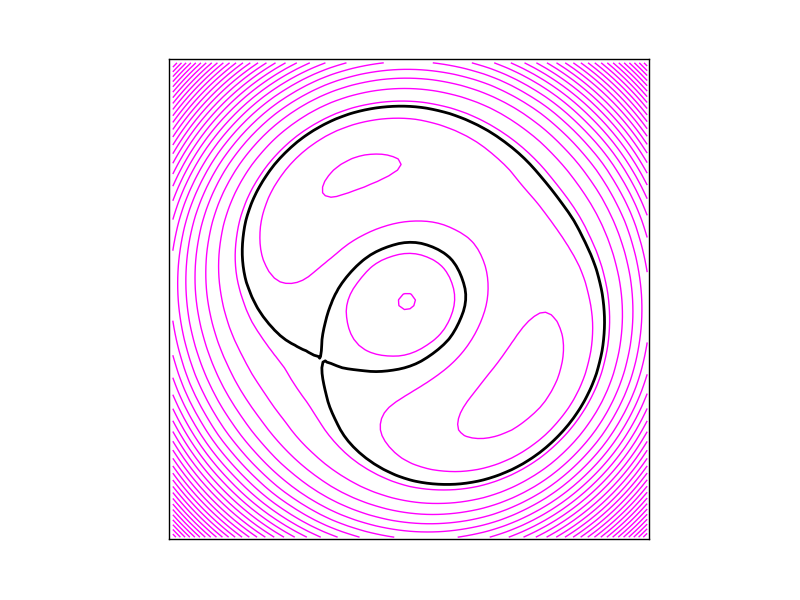
\includegraphics[width=.32\hsize]{ASW0000ar2_arriv.png}
\caption{A simple two-image lensed quasar.  The minimum and saddle are
  identified correctly.  The mean model shows two spurious images, but
  the mean convergence in the region of images is good.
\label{fig:ASW0000ar2}}
\end{figure}

\end{document}

